\chapter{Google Architecture}
\label{chap:google_architecture}

Google is one of the well-known examples of corporations that deal with Big Data.
Its activity directly relates to storing and processing of large volumes of data.
Google Search engine handles more than three billion searches every day.
Social networking service Google+ had 540 million users in 2013.
Gmail, Google's email service, had 425 million users in 2012.
These are just several examples of large-scale Google projects, that processes huge amounts of data.
Therefore, Google introduces a batch of solutions for building scalable systems. 

The overall structure of Google Big Data architecture is presented on the
Figure~\ref{fig:google_architecture}.
The lowest layer is Linux kernel, that serves as a basis for Google File System.
Google File System is a scalable and highly available file system. 
These properties are achieved by replicating data across several machines.
Next, data can be efficiently processed by MapReduce framework.
This technology includes two steps - map, that performs filtering and sorting and reduce, that aggregates the output of map step to the final result.
Bigtable, a highly scalable database, provides a way to store massive amounts of information.
Finally, client application uses these technologies to perform highly scalable and distributed tasks.  
Let us explain in more detail the primary features and internal structure of these technologies.

\begin{figure}
  \centering
  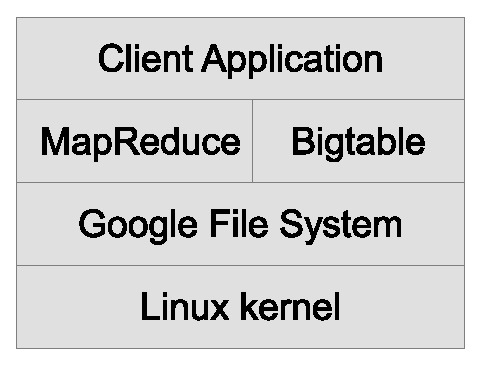
\includegraphics [width=0.4\textwidth]{images/Google_architecture}
  \caption{Google Architecture}
  \label{fig:google_architecture}
\end{figure}

\authorsection{Google File System}{SP}
[reference]
\mnote{Google File System}
Google File System (GFS) is a scalable distributed file system, which supports Big Data operations.
The underlying idea is the following: Google Search Engine and some other Google systems process vast amount of data, which is spread all over the world.
Hence the file system should be highly extensible, give an opportunity to use cheap hardware components and, consequently, be fault tolerate. 
Furthermore, it has some specific usage features.
Because of vast scales and cheap hardware, component failure is a commonplace.
The size of files exceeds several-fold the traditional standards, so a multi-gigabyte file is not unusual.
Most of the time the stored data stays unchanged and new data is only appended.
The append operation, in its turn, should provide the concurrent access for multiple clients.
GFS architecture design helps to meet all these requirements.

The Figure~\ref{fig:GFS_architecture} illustrates the main components of the GFS
Architecture.
Each GFS cluster contains one master server and several chunkservers.
The master has a "shadow" node, that provides read-only access when the primary master is down. 
Chunkserver stores chunks as Linux files on local disk.
Every chunk is replicated on several chunkservers for reliability.
One chunk combines multiple files and has a fixed size of 64 megabytes.

% Figure: according to [66]
\begin{figure}
  \centering
  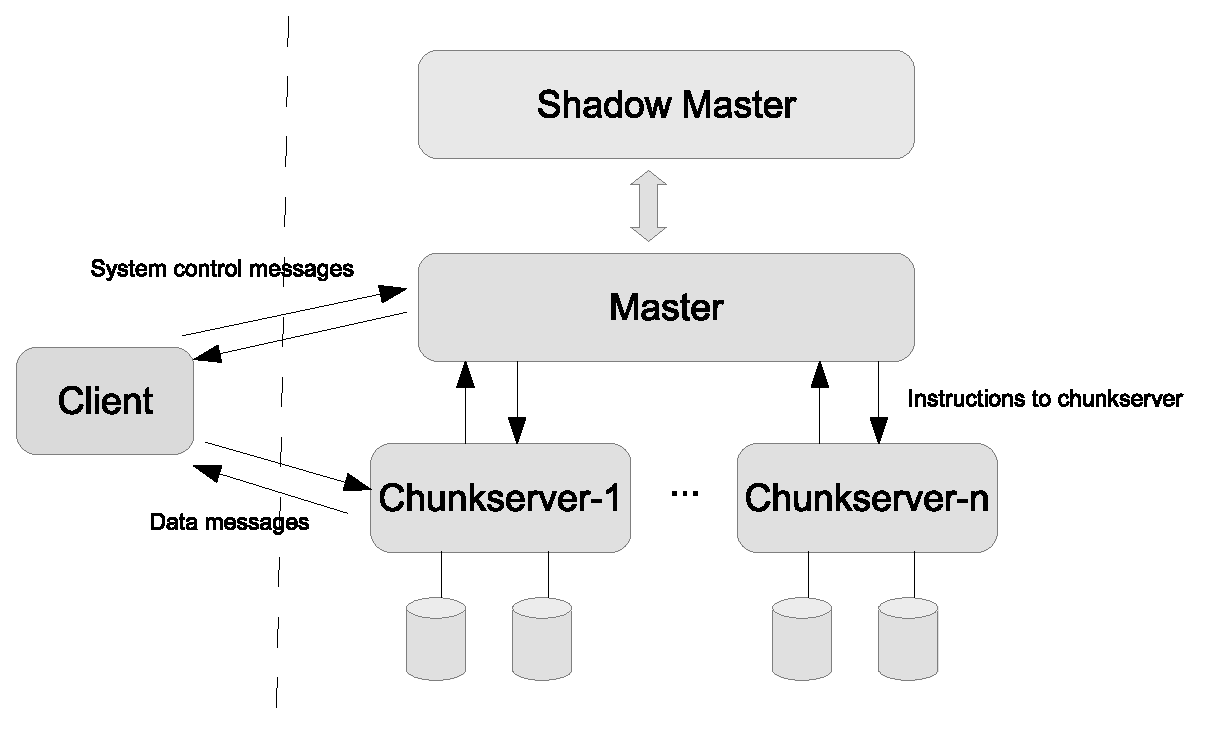
\includegraphics [width=0.8\textwidth]{images/GFS_architecture}
  \caption{GFS Architecture}
  \label{fig:GFS_architecture}
\end{figure}

The large size of chunk gives several advantages.
Clients send requests to the master for chunk location less frequently.
A persistent TCP connection to the chunkserver for a longer time period allows to avoid network overhead.
The master node stores less metadata that provide a possibility to keep it in memory.

The master node manages the mapping from files to chunks, location of chunks, access control, garbage collection and some other tasks.
It does not persistently store the information about chunks location. 
On the contrary, it gives instructions to chunkservers and collects their states using periodic HeartBeat messages.
To prevent the master being a bottleneck, only file system control data goes through it.
For example, a client can ask the master node which chunkservers it should contact.
The master node returns the corresponding chunk handle and its replicas' location.
After receiving a reply, the client caches this information and can directly transfer data to the given chunkserver, dispensing master node from overload.
Clients and chunkservers do not cache file data.
Clients mostly work with files that are too large to be cached.
Chunkservers treat chunks as Linux files, therefore in this case caching is done by operating system.

\mnote{Operation Log}
To recover its state, the master uses the operation log.
The operation log consists of the chronometric information about critical metadata changes.
This log is replicated on several machines.
For the purpose of consistency, client receives a respond for operation only when corresponding log record is flushed to a local disk and the disks of all replicas.
To avoid the operation log being too large, the master makes a checkpoint each time when the log size exceeds a certain threshold.
In the case of failure, the master can load the latest checkpoint from local disk and replay it, recovering its state.
For storing checkpoint it uses a compact B-tree like data structure, that allows to map it directly into memory and perform fast lookups.
For performance reasons the new checkpoint is created in separate thread.
The ability of a server to restore its state does not depend on the way it was terminated.
Shutting down a server by killing the process is a normal procedure. 

\mnote{Mutation}
A mutation denotes a change of the contents or metadata of a chunk.
There are two types of mutations, namely writes and record appends.
In the former case data is written with a file offset specified by a client.
In the latter, GFS chooses an offset, and data (record) is appended with an append-at-least-once semantics.
Record append operation is atomic, i.e. it is treated as one continuous sequence of bytes. 
This allows multiple clients to append information concurrently.

\mnote{Lease}
Each mutation is replicated across several chunks.
To keep a mutation order consistent at all the replicas, GFS uses a technique of leases.
The master gives a lease to one of the replicas, that becomes a primary replica.
The primary chooses an order for all the chunk's mutations and each replica then follows this order when applying mutations.

The flow of write control is shown on the Figure~\ref{fig:write_control_flow} in
more details.

\begin{figure}
  \centering
  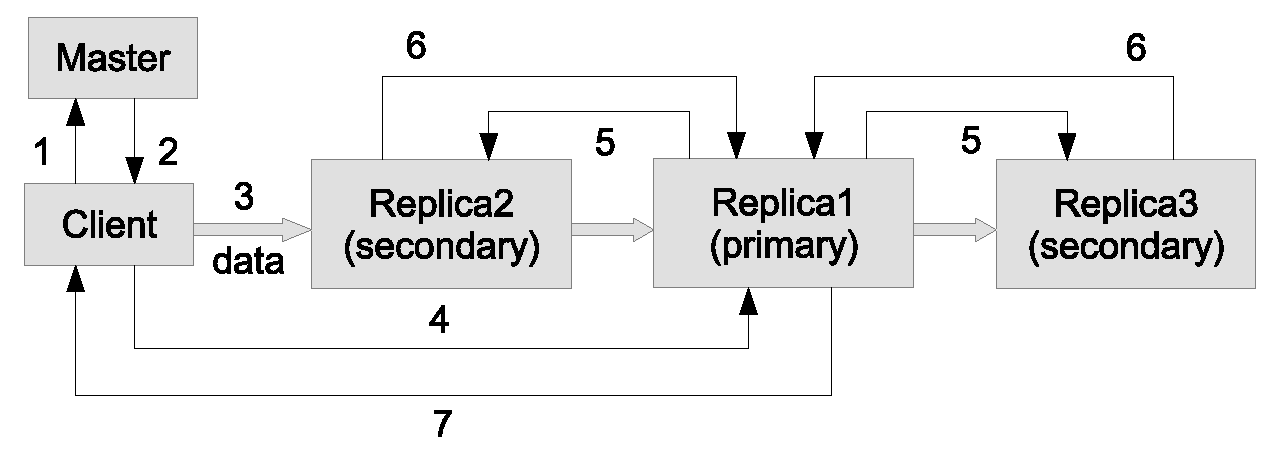
\includegraphics [width=0.7\textwidth]{images/write_control_flow}
  \caption{Write control flow}
  \label{fig:write_control_flow}
\end{figure}

1. The client sends a request to the master.

2. The master replies with a chunkserver, that holds the current lease, and the location of the other replicas.
If a primary replica (that has a lease) is not defined, the master chooses one. 
The client caches this information for the next mutations.

3. The client sends the data to all the replicas in arbitrary order.
Chunkservers store this data in an internal buffer cache. 

4. When the client receives acknowledgements from all the replicas, it sends a write request to the primary.
The primary picks serial numbers to all the mutations it has received and performs them in corresponding order.

5. All secondary replicas receive the write request forwarded by the primary.
Each replica applies mutations to its own state in the same order assigned by the primary.

6. The secondaries notify the primary about the completion of the operation.

7. The primary sends a reply to the client.
In the case of error occurrence at any of the replicas, the primary informs the client about them.
The write is considered to be successful, if the primary and an arbitrary number of secondary replicas succeeded.

GFS differs from traditional file systems in the way how it manages files and directories.
There is no possibility to list all the files in a directory in GFS, because it does not support per-directory structure.
It stores a mapping between full pathnames and metadata in a lookup table.
Prefix compression helps to efficiently represent this table in memory. 

The file deletion does not occur at once.
Firstly the master logs the event of deletion.
Than the system renames the file with a hidden name that includes the time of deletion.
The master performs a regular scan of the namespace and removes a hidden file, if it has existed for more than a specified time interval (e.g. 3 days). 

All the described features help the Google File System to successfully cope with a large-scale data processing workload.
GFS meets the storage needs of Google corporation.
Therefore Google uses GFS as the storage platform for many applications, both in research and production areas.
Another Google technologies, like MapReduce or BigTable are based on it.  	 

\authorsection{MapReduce}{SP}
[reference]
MapReduce model finds wide application in a variety of real world tasks.
For example, search engines use web crawling to gather a vast amount of information.
They process this information to create inverted indices, construct web graphs, figure out the most frequent search queries, etc.
Any of these tasks can be divided into two steps, namely Map and Reduce.
Map operation converts input data to a set of intermediate key/value pairs.
Reduce operation, in its turn, combines all the values that share the same key.
The advantage of the MapReduce abstraction is that it hides the implementation details from users.
This allows even not experienced programmers to easily construct parallel and distributed systems.

MapReduce shares the same requirements with other systems that work with large data sets.
It should provide high parallelization, be fault-tolerant and perform load balancing between nodes.
Applying Map and Reduce operations helps to parallelize large calculations.
Moreover, this makes simpler re-execution of a task that serves as a primary mechanism for fault tolerance.

Both Map and Reduce operations work with key/value pairs.
The user of MapReduce library determines the logic of these operations, specific to the given application.
The Map function receives an input a key/value pair and produces a set of intermediate pairs.
The MapReduce library groups these intermediate pairs together by the key and passes the result to the Reduce function.
It passes them via iterator that allows to handle a large data set without keeping it in memory.
The Reduce function merges the values with the same key, possibly decreasing a given set of values.
One Reduce function invocation most of the time produces a single output value, or even none.
A pseudo-code for a simple MapReduce task is illustrated in Listing~\ref{lis:simple_mapreduce_task}.

\begin{lstlisting}[caption=Simple MapReduce task, label=lis:simple_mapreduce_task]
def map(key, value):
	list = []
	for x in value:
		if some_condition_holds:
	 		list.append((key, x))
	return list

def reduce(key, list_of_values):
	result = 0
	for x in list_of_values:
		result += x
	return (key, result)
\end{lstlisting}

\begin{figure}
  \centering
  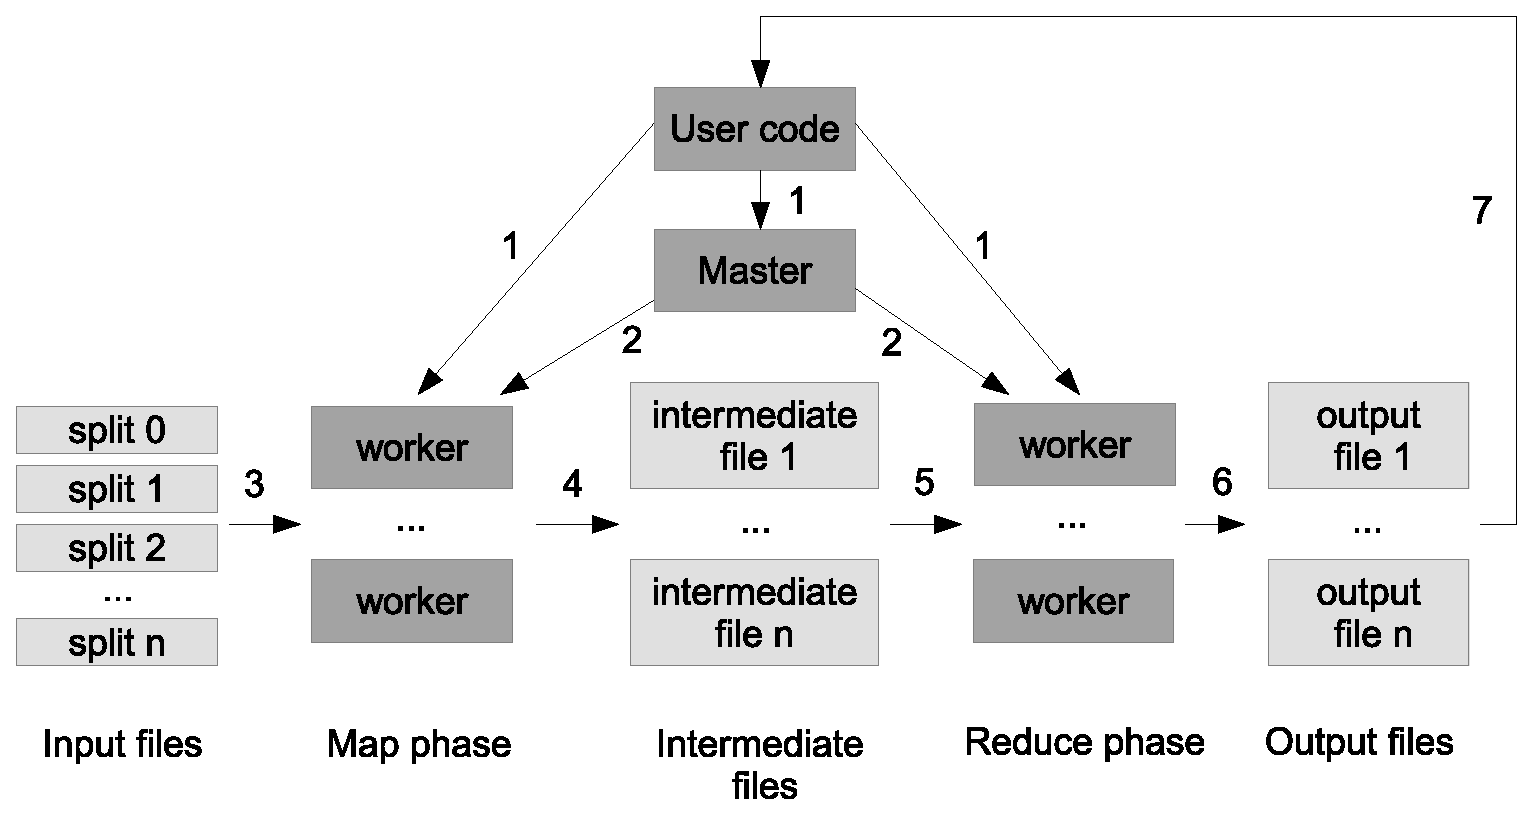
\includegraphics [width=0.9\textwidth]{images/MapReduce_operation_flow}
  \caption{MapReduce operation flow}
  \label{fig:mapreduce_operation_flow}
\end{figure}

We visualize the overall flow of a MapReduce operation in the Figure~\ref{fig:mapreduce_operation_flow}.

1. The MapReduce library divides the input files into M splits.
The size of one piece varies from 16Mb to 64Mb depending on the chosen settings.
User code invokes the MapReduce routine on several machines.

2. One of these machines is a master, while others are workers.
The master manages the workers, assigning to idle nodes one of M map tasks or one of R reduce tasks.

3. A worker that handles a map task reads the data from a respective input split.
It passes the parsed key/value pairs to the Map function.
The intermediate output of the Map function is stored in a buffer.

4. The MapReduce library periodically writes the buffered data into selected number of R local intermediate files.
Also it informs the master about the location of these files.

5. The master passes the locations to workers that handle a reduce operation.
A reduce worker reads the intermediate pairs from a specified location using remote procedure calls.
After compliting the reading, the worker groupes together all the pairs that share the same key.

6. These pairs are then passed to the Reduce function, one key and one or several related values at a time.
The output of the Reduce function is written to one of the output files.

7. After finishing all the map and reduce tasks, the MapReduce library returns the control to the user code.
The derived output files can be directly processed or be used as an input to another MapReduce task.

The MapReduce library has an optional Combine function that can be used for optimisation.
For example, let us consider the task of counting the number of words in English text.
Most probably it contains a lot of articles `a` and `the`.
Each Map task sends thousands of pairs <a, 1> to a single Reduce operation over the network. 
The Combine function can improve this situation by partial merging these pairs before sending them over the network.
Each machine that executes a Map function now also executes a Combine function.
Combine operation often uses the same code as Reduce one.
The difference is that the output of the former is stored in an intermediate file, while the latter writes it into the final output file.

The usage of Google File System (GFS) for storing input data helps to reduce the network bandwidth consumption.
GFS stores input data in blocks, copying each block on different machines (usually it makes 3 copies).
The master in MapReduce library knows which machine contains a replica and tries to assign a corresponding map task to this machine.   
When it is not possible, the master uses the nearest node to that machine.
This technology conserves network bandwidth significantly, especially when dealing with huge MapReduce operations.
 
The master keeps track of worker failures.
For this purpose it stores the state of each task and the identity of the worker that performs the task.
There are three types of states: idle, in-process and completed.
The behavior of the master in the case of failure depends on the type of the task (map or reduce) that failed.
When the map task fails, the master re-executes it on another worker.
Re-execution is required since the output of the map task is stored locally on the failed machine.
On the contrary, there is no need to re-execute the reduce task because global file system stores its output.
Sometimes a failure is caused by a defective record.
In this case the MapReduce library optionally can skip this record to continue the work. 
 
Stragglers is another problem that can obstruct the task completion.
Straggler is a machine that handles the last several map or reduce tasks too slow, keeping the whole system waiting for completion.
The MapReduce master uses a special mechanism to solve this problem.
On termination of an operation it executes the remaining in-process tasks on two different machines.
When either primary or backup worker completes computations, the task is considered to be completed.

Google Search engine widely uses MapReduce functionality for indexing, computing different statistics and analysing data.  
Moreover MapReduce can significantly facilitate the problems of data mining and machine learning.
Its key feature of dividing the computation into Map and Reduce phases helps to easily build distributed systems and makes the computation considerably more efficient.  

\authorsection{BigTable}{SP}
[reference]
Some Google projects deal with so large amounts of data, that common storage systems cannot sustain such a load.
For instance, personalized search, that stores user browser history and handles search queries based on the stored information about user activity.
It is necessary to warehouse each user's data.
Taking into account the huge number of Google Search users, the amount of data to be stored is also tremendous. 

The company introduces its own storage system for these purposes - a Bigtable.
It is a sparse, distributed, persistent multidimensional sorted map. [reference]
Bigtable uses three-dimensional mapping: row key, column key and timestamp are mapped to an array of bytes.
It is created to store petabytes of data in a distributed way.
As Google uses Bigtable in various projects, it puts different requirements on data size and latency of the storage system. 

\mnote{row keys}
The row key is represented by an arbitrary string with a maximum size of 64Kb.
Read and write operations under one row key are atomic.
Bigtable stores row keys in lexicographic order and dynamically partitions each row range.
One partition is called a tablet and serves as a distribution and load balancing unit.
For instance, when storing web pages with an URL as a row key, it is optimal to arrange pages from the same domain in one tablet.
In this case an URL like en.wikipedia.org/index.html is presented as org.wikipedia.en/index.html.

\mnote{column keys}
Bigtable groups column keys into column families, which serves as an access control units.
It means that each column family can have different access permissions (e.g. write access for one application and read only for another one).
It is common to store in one column family data of the same type.
One can store data under a column key only when a column family comprising this column key is created.
Number of distinct column families should be kept small, while each column family can contain unbounded number of columns.
The name of column key is presented as family:qualifier pair, where family should be printable and qualifier can be an arbitrary string.
For example, the column key name can look like language:en, where 'language' is a column family name and 'en' is a language ID. 

\mnote{timestamps}
Timestamps are used to store multiple versions of the same information.
A timestamp can be assigned in different ways.
On the one hand, Bigtable can use the time in microseconds as a timestamp.  
On the other hand, a client application can maintain its own unique timestamps.
Several versions of data are ordered such as the most recent version can be accessed first. 
Garbage collector processes the outdated data automatically using one of the two column family settings to detect the outdated versions.
The first setting allows to keep only the last \textit{n} versions of data, while the second setting allows to keep data that was written in the last \textit{m} days.

\mnote{Sawzall}
Bigtable allows user to manipulate the stored data using a special language developed by Google.
The language is called Sawzall.
Scripts, written in this language, can execute on Bigtable server's address spaces.
Using Sawzall scripts one can filter, transform and make various summarization on data.

\mnote{Chubby}
Chubby is a persistent distributed lock service for synchronizing access to shared system resources.
The Chubby service replicates to five nodes, choosing one of them to be a master node.
The service provides a namespace, that contains directories and files, and uses them as a lock.
Chubby has a client library that can keep the cached Chubby files in memory.
Every client sustains a session with Chubby service.
The expired session loses all the locks.

Bigtable uses Chubby for several purposes.
First, Chubby guarantees to have at most one active master at a time.
Second, it handles the appearance of new tablets and finilizes the dead ones.
Third, it stores the schema of Bigtable and access control lists.

The major components of Bigtable are a master server, a number of tablet servers and a library linked into each client.
It is possible to dynamically add or remove tablet servers according to given workload.
The master assignes tablets to tablet servers, performs load-balancing, garbage collection.
Furthermore, it is responsible for creation of tables and column families.
Each tablet server controls a tablets set.
When a client sends a read or write request to the tablet, this request is processed by the tablet server.
Also the tablet server splits too large tablets.

The internal details of master-slaves interaction are similar to those mentioned above in GFS and MapReduce subchapters.
Analogously, the system does not transfer client data through the master and establishes a direct connection between clients and tablet servers.
It prevents the high load of a single master node.

A Bigtable cluster warehouses one or several tables.
A table contains a number of tablets. 
All the data that belongs to one row range is situated in one tablet.
Primarily one table contains only one tablet.
When the table becomes larger than a specified threshold, it automatically splits into several tablets.

\mnote{METADATA table}
The root tablet uses a special METADATA table to store the location of tablets.
The root tablet is a first tablet in this table.
However, it is never split in contrast to the rest of the tablets to keep the number of hierarchy levels constant.
Figure~\ref{fig:bigtable_tablets_hierarchy} illustrates the tablets hierarchy.
The METADATA table also stores logs of operations on each tablet.
This data can be used for preformance analysis and debugging.  

\begin{figure}
  \centering
  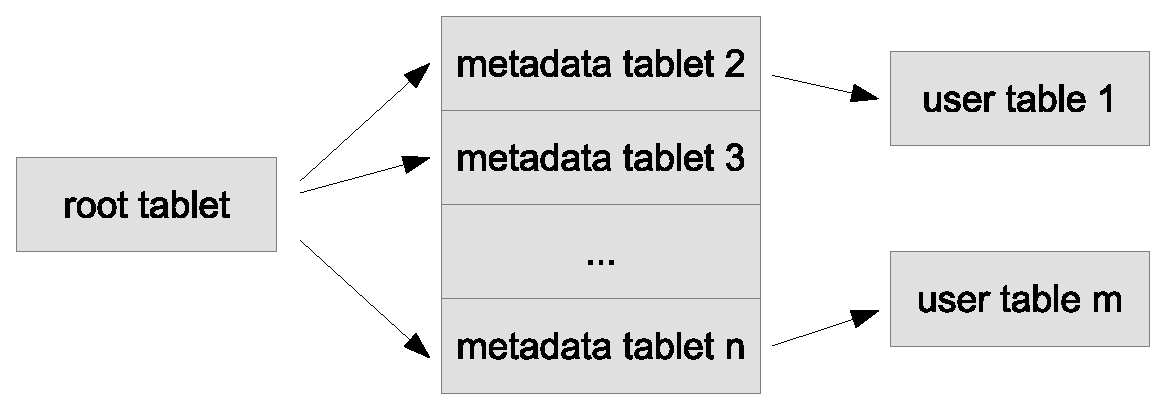
\includegraphics [width=0.7\textwidth]{images/bigtable_tablets_hierarchy}
  \caption{Bigtable tablets hierarchy}
  \label{fig:bigtable_tablets_hierarchy}
\end{figure}

\mnote{SSTable}
Bigtable stores data in special file format called SSTable.
Each SSTable consists of several blocks of a fixed size (64Kb by default). 
To locate blocks it stores their indexes, that are loaded into memory on opening the SSTable.
The blocks indexes considerably decrease the lookup time.
First the binary search is performed on in-memory index to find the needed block.
Than the appropriate block is read from disk.
The whole SSTable can be loaded into memory if necessary to perform lookup and scan operations avoiding touching disk.

A tablet can be recovered using a commit log.
This log contains all the tablet updates.
The most recent updates can be obtained from a memtable - a sorted buffer in memory.
The set of SSTables stores the older updates. 
A tablet server can read the METADATA table to detect the necessary SSTables for recovering.
Than the tablet server applies all the updates in order to restore the crashed tablet. 
  
A tablet server checks the incoming read and write operations.
The operation should be well-formed and the sender should be authorized to perform a mutation.
First the server writes a valid mutation to the commit log.
Then for write operation it inserts its content to memtable.
When the size of the memtable goes beyond the given threshold, the system frozes it.
It creates a new memtable and converts the frozen one into an SSTable. 
Read operation is performed on a merged view of the memtable and corresponding SSTables.

Periodically a merging compaction on SSTables and the memtable are used to create new SSTables out of old ones.
A regular compaction merges the memtable and a few SSTables, keeping the deletion information and deleted data.
A major compaction merges all SSTables into exactly one SSTable, cleaning deletion entries.
Bigtable performes the compaction mechanism regularly to keep the system up-to-date.

The variable number of tablets makes the system flexible and therefore easy to scale.
The implementation features provide good performance and high availability.
Bigtable is successfully used in many Google products, that proves the high quality of this storage system.

% Other BigData systems:
%Malewicz - Pregel
%Melnik - Dremel
%Akidau - MillWheel

\authorsection{Facebook architecture}{SP}

Facebook is another representative company that is strongly connected with Big Data storing and processing.
The main difference is that Facebook applications often require real time data processing, providing a user with immediate feedback.
On the contrary, for most Google applications batch processing is sufficient to make necessary computations.

% add intro about HDFS, Hive, etc.

Facebook widely uses such technologies for distributed data warehousing and computation as HDFS, Hive and Scribe. 
While HDFS is an exterior module, Hive and Scribe were initially developed at Facebook and only later became open-source under the Apache Software Foundation.

\mnote{Hive}
Hive is a framework designed for storing data.
Facebook uses it for making queries and perform data analysis.
Hive provides SQL-loke interface 



% Scribe

\mnote{Facebook architecture}
Figure~\ref{fig:facebook_data_flow} demonstrates the data flow in Facebook architecture.
Data originates from two sources: web servers and federated MySQL instances.
Web servers generate log data, that consists of variuos events, e.g. a user clicked a link or 'liked' a photo.
The federated MySQL contains the descripting data, such as the time of posting the link and the place where it was done.

\begin{figure}
  \centering
  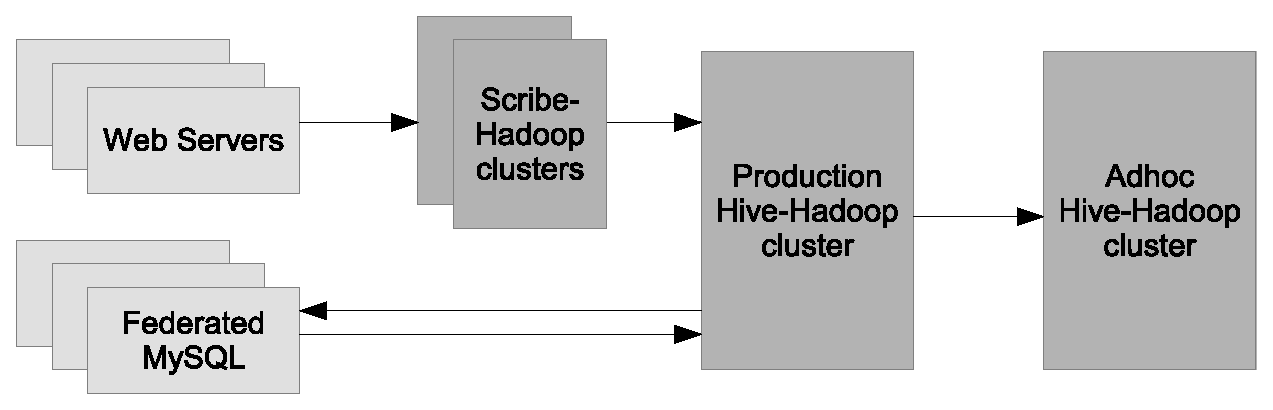
\includegraphics [width=0.8\textwidth]{images/facebook_data_flow}
  \caption{Data flow in Facebook}
  \label{fig:facebook_data_flow}
\end{figure}

Data flow goes from web servers to Scribe-Hadoop clusters.
Such cluster is actually a Hadoop cluster with a running Scribe server on the top of it.
The main function of Scribe is to aggregate the input data and write it into HDFS.
This data is transferred uncompressed [Data Warehousing and Analytics Infrastructure at Facebook] that can be a bottleneck for the whole system.
Facebook alleviates the problem by putting Scribe-Hadoop close to web servers, decreasing the network transfer load.
Periodically Scribe-Hadoop clusters send compressed data (mostly as HDFS files) to Hive-Hadoop clusters.
It is loaded to Hive and becomes available for other modules.

Scrape processes load data from federated MySQL to Hive-Hadoop cluster.
They get a dump of needed data from database, compress it and move it to the cluster.
This process should be resilient and avoid putting extra load on the databases.
The former is accomplished by using the previous days data when the database is not reachable at the moment.
To meet the latter requirement, scrape process runs on a MySQL database replica.

There are two types of Hive-Hadoop clusters - a production cluster and an adhoc one.
The purpose of the production cluster is to execute high prioriy tasks with strict deadlines.
On the contrary, the ad hoc cluster processes batch jobs with low priority and makes ad hoc analysis.
These tasks are separated, because it can be dangerous to run ad hoc user query on a production cluster.

When the data is needed for both clusters, it is replicated from the production to the adhoc cluster.
It is done in this order, because the data should be available earlier for critical jobs on the production server.
Moreover, the production server is more reliable.
During the replication process the data is transferred in a raw form accompaned by the respective metadata.

The stored data can be either transformed or queried by users.
Most of the time Hive-Hadoop clusters keep the data for future analysis.
However, in some cases the federal MySQL tier gets the data back.
This data can be uploaded on the Facebook site and participate in the further interaction with Facebook users. 





% 1. Flow of data (Data Warehousing and Analytics Infrastructure at Facebook)
% 2. HDFS enhancement + HBase + Hive + Scribe (Data Warehousing and Analytics Infrastructure at Facebook) + (Apache Hadoop Goes Realtime at Facebook)
% 3. Haystack (https://www.facebook.com/note.php?note_id=76191543919) + (Finding a needle in Haystack: Facebook�s photo storage)
% 4. jemalloc (https://www.facebook.com/notes/facebook-engineering/scalable-memory-allocation-using-jemalloc/480222803919)